%----------------------------------------------------------------
%
%  File    :  introduction.tex
%
%  Author  :  Olli-Pekka Riikola, TU Graz, Austria
% 
%  Created :  3 Dec 22
% 
%----------------------------------------------------------------


\chapter{Introduction}

The great idea behind the World Wide Web is that it connects people
all over the world, and almost everyone is able to access it. But it
is only almost. Of course there are places where the internet is not
freely available and due to restrictions or poor connection it is not
possible to access it at all but there are also different
situations. Could be that there are no restrictions for accessing the
internet or the internet connection is not poor, but still some users
cannot access the web. Why is that?

Even though there now are great information infrastructures in the
states and cities and there are those good looking websites in there,
also there is still a great drawback in the terms of web accessibility
- a poor web design. For example visually-impaired users cannot really
see all the beautiful content or extremely diverse navigation bars,
but rather they will struggle through the endless link lists, one by
one, trying to figure out what is going on in the website. It is true
that they have some assisting devices, like a device for the Braille
reading or software for text to speech but there is one common factor
with these all. It is necessary to read the screen somehow and there
comes the problems.

The problems that blind users may face are empty element attributes or
empty link lists in the site, dynamic content or other elements which
are difficult to read by screen readers. They might look like very
tiny problems, but in reality they are remarkable accessibility issues
when we are talking about visually-impaired users. Luckily, as
mentioned above, there are tools for both visually-impaired users and
web developers to escape these problems. Blind users can use a text
browser in combination with screen reader and the developer can use
accessibility checking tools to ensure that a website will be properly
accessible at the end. And these tools are what this paper is about -
checking web accessibility.

Throughout the whole paper there will be two websites as examples of
accessibility. The first one is www.gov.uk which represents a good
example of an accessible website. Another one is www.mirror.co.uk
which is a bad example of accessibility - can even be said that it is
a good example of bad web accessibility.


\begin{figure}[tp]
    \begin{minipage}{0.48\linewidth}
        \centering
        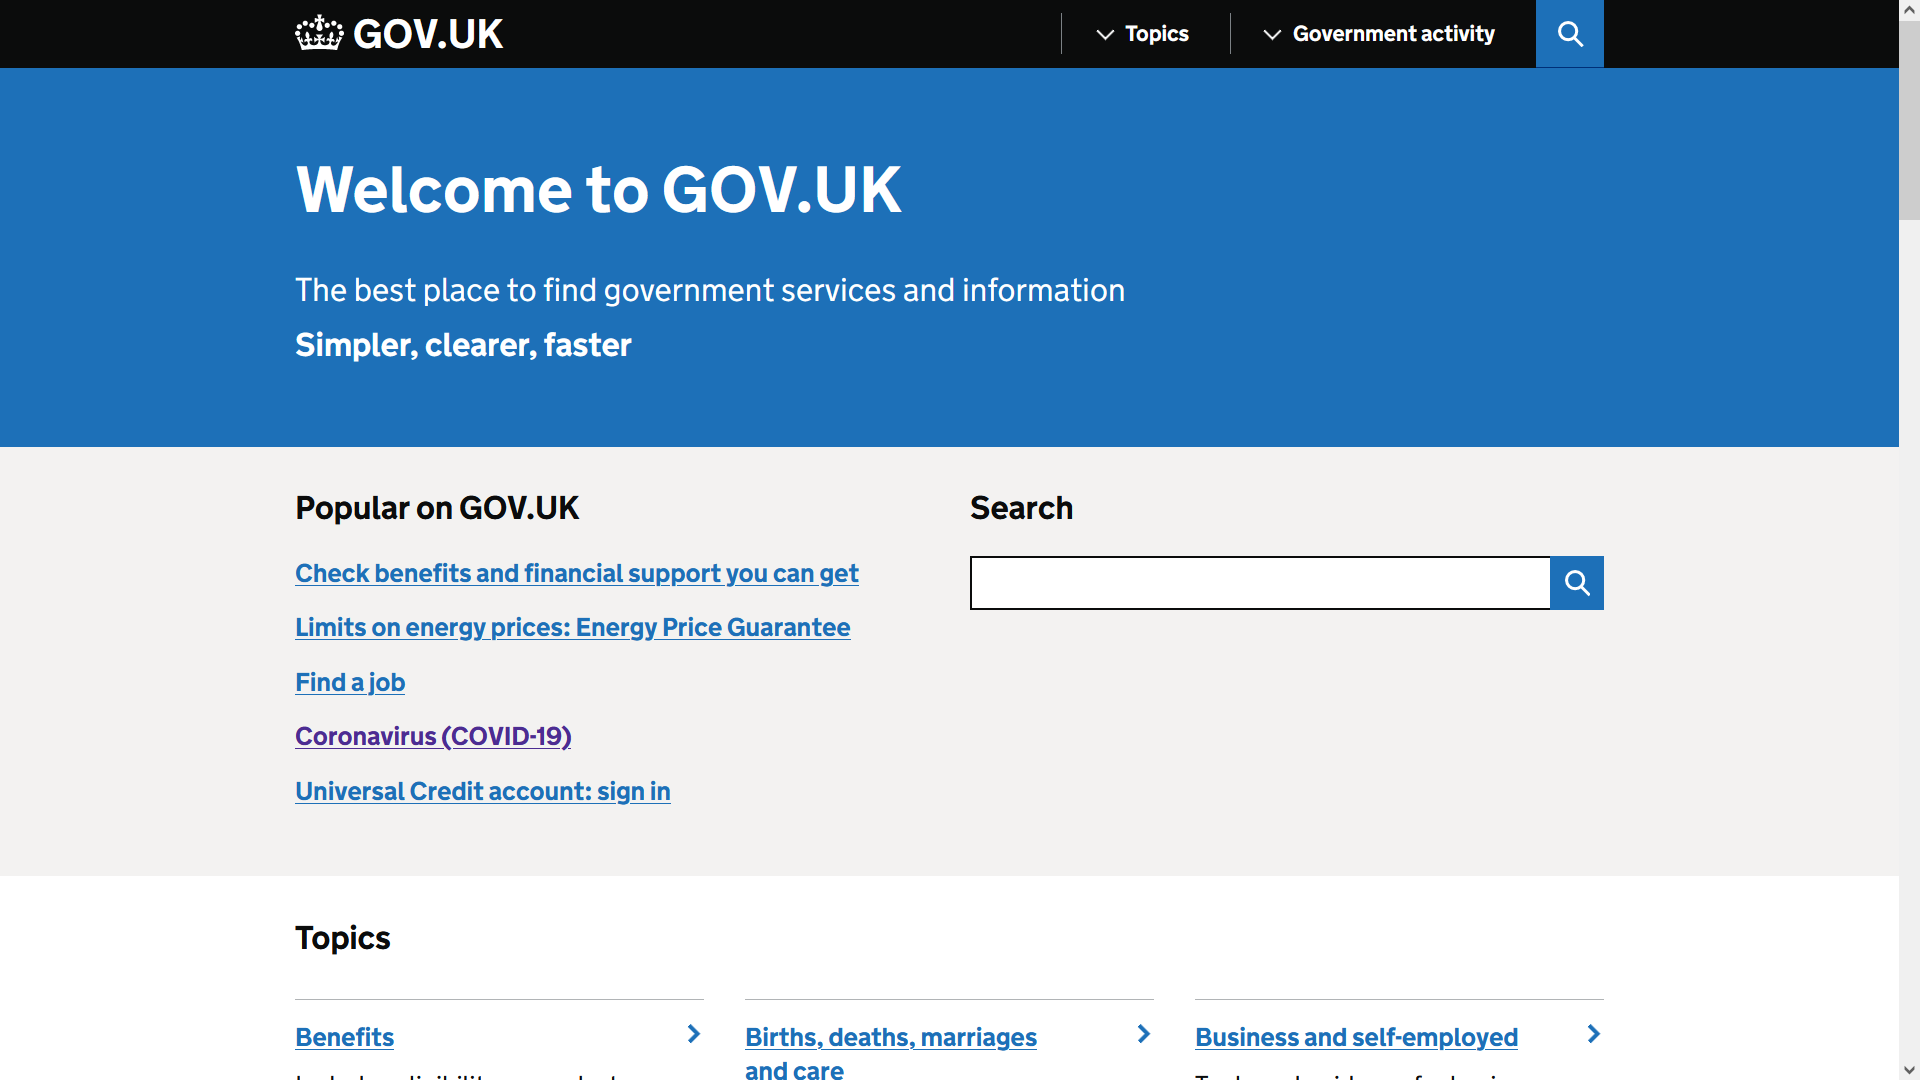
\includegraphics[keepaspectratio,width=\linewidth]
        {images/gov}
        
        \caption[www.gov.uk]
        {%
        This website is good example of accessible website.
        }
        \label{fig:gov}
    \end{minipage}\hfill
    \begin{minipage}{0.48\linewidth}
        \centering
        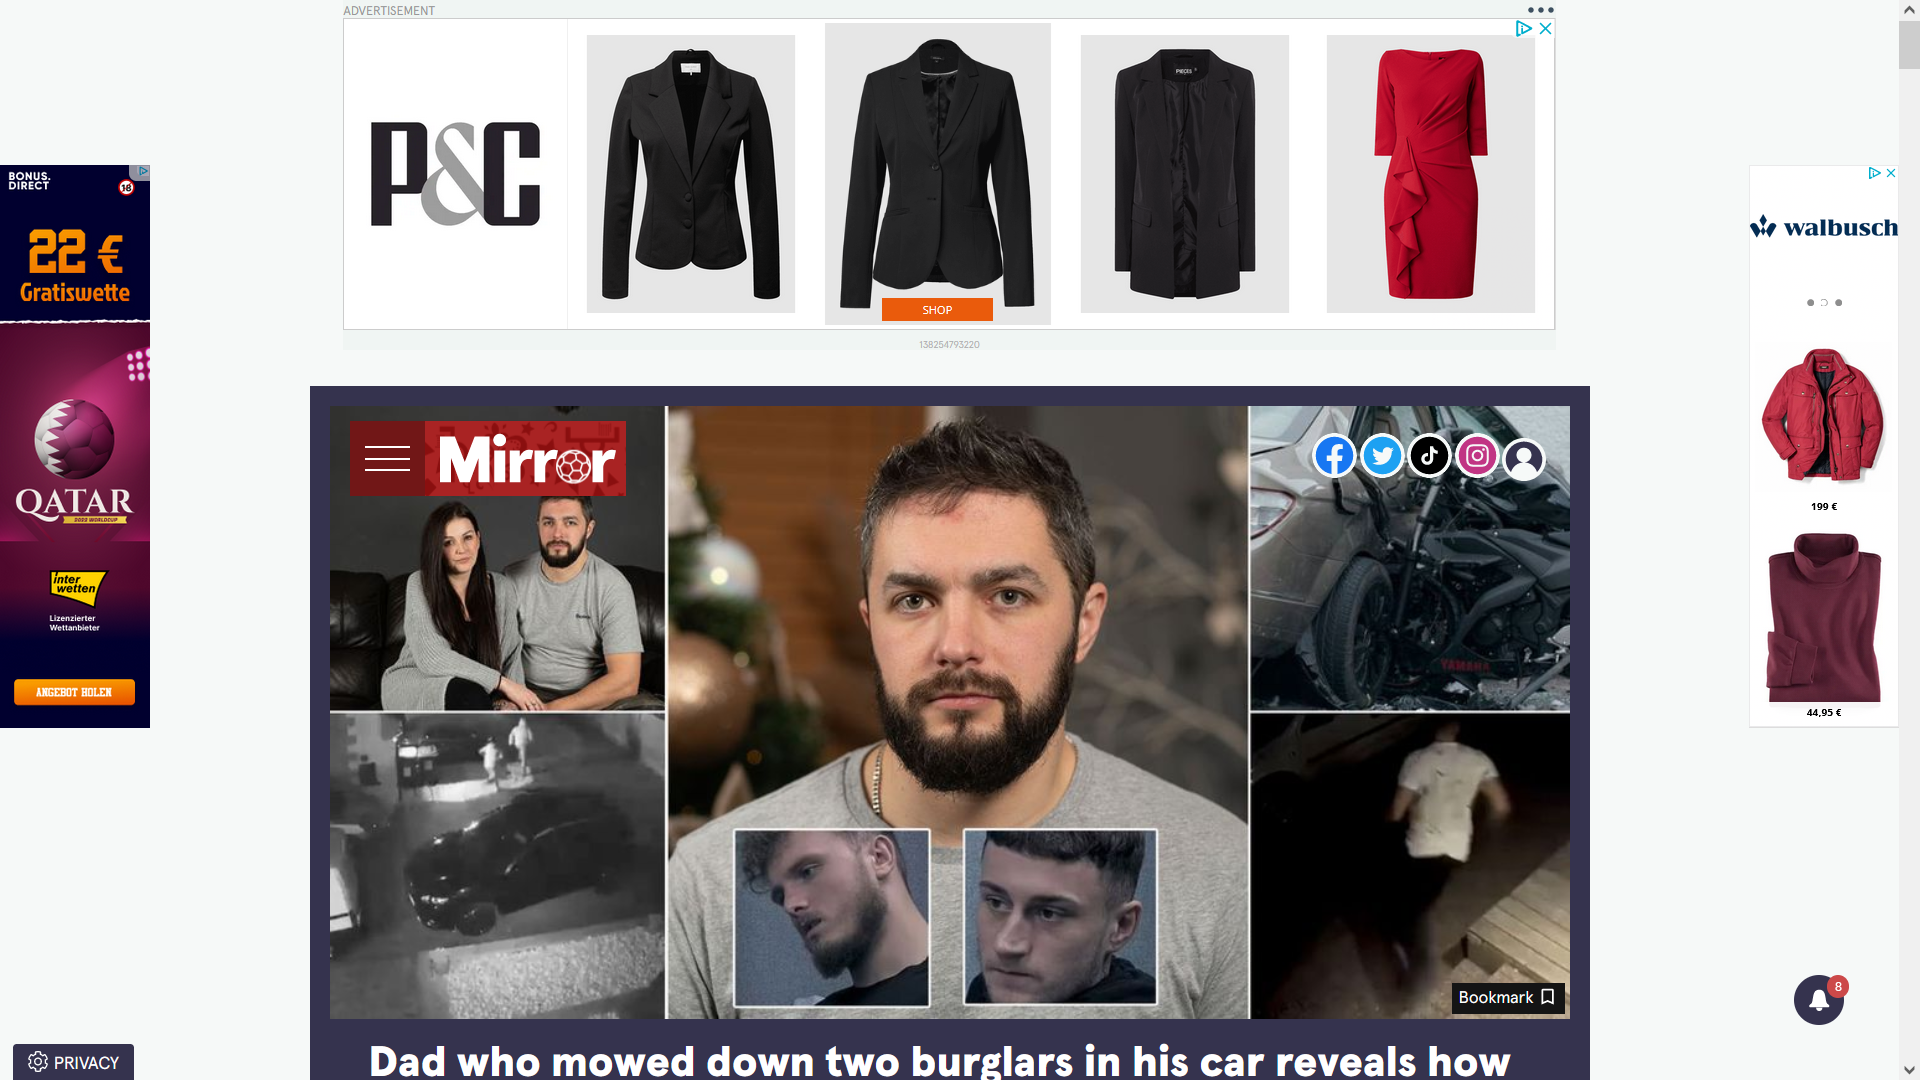
\includegraphics[keepaspectratio,width=\linewidth]
        {images/mirror}
        
        \caption[www.mirror.co.uk]
        {%
        This website has quite a poor accessibility.
        }
        \label{fig:mirror}
    \end{minipage}
\end{figure}
